\documentclass[11pt]{article}

%\usepackage[pdftex]{graphicx}
\usepackage{graphicx}
\usepackage{fullpage}
\usepackage{amsmath} %for align
\usepackage{hyperref} %for url
 \usepackage{color} %for color

%\providecommand*\emaillink[1]{\nolinkurl{#1}}
%\providecommand*\email[1]{\href{mailto:#1}{\emaillink{#1}}}

%\usepackage{etoolbox} %used by toggle
%\newtoggle{answers}
%%\togglefalse{answers} %set this if you *do not* want the given toggle.
%\toggletrue{answers} %set this if you want the given toggle.
%

 \def\bluehref#1#2{\href{#1}{\color{blue} #2}}    

\begin{document}\begin{center}
{ \Large \bfseries IEEE Control Systems Society Education and Outreach @ UTSA}\\[0.4cm]
{ \large \bfseries Day \#2}\\[0.2cm]
\center{ \bfseries Line Following Robot, More Sensors and programming, Parallel parking}
\end{center}

%\noindent  \textcolor{red}{
%\bf PLEASE READ THIS:} {After the lab grading is done, please return your boxes to BSE 2.216. When returning your boxes, please provide a list of items (e.g., technic elements, brick, sensors, motors) that are missing/broken or extra pieces that might have ended in your boxes. We will not penalize you for breaking or missing pieces. Your diligence in reporting will help us to replace those parts before we hand the kits to student next time. Many thanks. -Pranav}

%\section{Expectations}
%If you lose any parts or break anything, please let the TA know and send an email to the instructor with the part number: %\email{pranav.bhounsule@utsa.edu}{pranav.bhounsule@utsa.edu}. 
%\href{mailto:pranav.bhounsule@utsa.edu}{pranav.bhounsule@utsa.edu}.
%This will help us to order for replacement before we give our the LEGO sets next time the course is offered. 
%\\
%\\
%You are supposed to work on the labs in groups of 2 or 3. Each team member is supposed to participate in the programming. The TA/instructor at their discretion might ask any student to explain how a particular task was accomplished and use this to assign a grade. So please work together and contribute to the lab.

%\section{Equipment list}
%Here is webpage that tells you what the various components of the kit are able to do: 
%\bluehref{http://www.lego.com/en-us/mindstorms/products/31313-mindstorms-ev3}{http://www.lego.com/en-us/mindstorms/products/31313-mindstorms-ev3}
%\begin{itemize}
%\item {\bf Computer:} 1 NXT Brick and 1 USB cable to connect brick to your computer.
%\item {\bf Actuators:} 3 servo motors
%\item {\bf Sensors:} 1 Color sensor, 1 Gyro sensor, 1 Sound Sensor, 1 Ultrasonic Sensor, 2 Touch Sensor, 1 Infra red beacon, 1 Infra-red sensor, Cables to connect sensors to bricks
%\item {\bf Battery:} 1 Rechargeable battery and charger
%\item {\bf Boxes:} 1 LEGO expansion set and 1 LEGO Core set. Information about parts is here \bluehref{https://education.lego.com/en-us/lesi/support/product-support/mindstorms-education-ev3/ev3-expansion-set/element-surveys}{https://education.lego.com/en-us/lesi/support/product-support/mindstorms-education-ev3/ev3-expansion-set/element-surveys} 
%\end{itemize}

%%%%%%%%%%%%%%%%%%%%%%%%%%%%%%%

%\begin{enumerate}
%\item Find the other sensors in the kit. A list is given above.
%\item Try to write at least one program per sensor to learn about how it works.
%\end{enumerate}
%\section{Homework}

%\vspace{1cm}
\noindent This handout can also be found on this weblink: \bluehref{http://tiny.cc/ieee\_day2}{http://tiny.cc/ieee\_day2}

\vspace{0.5cm}
\noindent \textcolor{red}{\bf\Large Day 2, Session 1: 9:30 AM -- 12:00 PM} 

\section*{Task 1: Line Following Robot}
\paragraph{Motivation:} \bluehref{https://en.wikipedia.org/wiki/Automated_guided_vehicle}{Automated Guided Vehicles} (AGV) are used in manufacturing facility and warehouses to move equipment, people, and material. These AGV's follow predefined lines marked on the floor to navigate. 

\paragraph{Goal:}
In this lab, you will build and program a line following mobile robot that can go from a predefined start to a predefined end point in the given time. You will be evaluated based on how well you can follow the given line in a set amount of time. 
 
%\paragraph{Trajectory:} The trajectory can be downloaded here: \\
%\bluehref{http://engineering.utsa.edu/~pab/info/lego/lego\_trajectory1.pdf}{http://engineering.utsa.edu/~pab/info/lego/lego\_trajectory1.pdf} (0.2 MB) \\
%To use the map to practice open the file in Adobe Reader. Then go to Print $->$ Print as Poster (scale = 100\%). This will print the pdf on 8 letter size pages. You can then tape the pages on the ground to make a complete trajectory. Try to think of how you will get the robot to do the task. This will inform the next step.
%\noindent
%
\paragraph{Building an autonomous (not tele-operated) mobile robot:} Build a mobile robot that can turn and incorporate the color sensor that will enable the robot to see the line. Feel free to reuse the design you used earlier. Here is an example mobile robot but feel free to use your own design or customize this one: \\ \bluehref{http://aux.coe.utsa.edu/~pab/info/lego/lego\_vehicle.pdf}{http://aux.coe.utsa.edu/~pab/info/lego/lego\_vehicle.pdf} (5.4 MB)

%\paragraph{Practise Track:}
%\begin{enumerate}
%\item The TA will set up a practise track for you to practise. %There will be a different trajectory on the grading day. 
%The trajectory can be downloaded here: \\
%\bluehref{http://aux.coe.utsa.edu/~pab/info/lego/lego\_trajectory2.pdf}{http://aux.coe.utsa.edu/~pab/info/lego/lego\_trajectory2.pdf} (0.2 MB) \\ 
%To use the map to practice, open the file in Adobe Reader. Then go to Print $->$ Print as Poster (scale = 100\%). This will print the pdf on 12 letter size pages. You can then tape the pages on the ground to make a complete trajectory. 
%\item 
%\item Tele-operation (remote controlling the car) is not allowed. The robot needs to be autonomous (by itself).
%\item  
%\end{enumerate}

\paragraph{Tasks}
%The grading will take place in the classroom. Please arrive by 1:15 PM and be ready to demonstrate your robot. Ensure that the batteries are charged. 
%\subsection{Before you show up at the BSE atrium}
\begin{enumerate}
\item Your robot should use only the color sensor for this task. No other sensors are allowed.
\item Your robot needs to follow the black continuous line at all times. We will also keep a track of the time from start to end. HINT: Here is a tutorial on programming a line following robot: \bluehref{https://youtu.be/ODAGVeeDagk}{https://youtu.be/ODAGVeeDagk}
%\item For the competition, the TA/instructor will have a different course with similar level of difficulty.
\item One person from each team will place the robot in the orientation of her/his choice at the start point (which will be clearly marked). When the TA/instructor says, `Ready-Set-Go', the team member will press a button on the brick to get the robot moving. Your time will start when the TA/instructor says `Go'. Your robot has to follow the line from start to end. 
\item If your robot does not reach the finish (end of the line) you will get zero points. 
\item If you robot does reach the finish (end of line) then your score will be computed using the formula, Score = 100 - T, where T is the time taken by the robot from start to finish in seconds.
\item You will have three attempts to improve your scores.
%Points will be awarded for reaching each of the check points in that order. If the robot skips a checkpoint but return to the line afterwards, you will not be awarded points from there on. TA/instructor decisions are final.
%The total score for this part is 100 points. You have to complete the entire course in 20 seconds. If your robot takes more than 20 seconds, then there is a 20 points penalty. %{\bf (80 points)}.
%\item The TA will record your score and the time taken. In order to be declared a winner, the team that scores 100 points and takes least amount of time is the winner. 
%\item Only 1 team from the entire classroom will be eligible to win the grand prize. 
%\item Lab report (per group) is due by the end of the day the lab is graded. {\bf NOTE: Please look at some example lab reports posted on blackboard. Please go through them and my comments for the report. Please use them as a template to help you write the report for this lab. Grading will be stricter this time.} Suggested report size is 2 pages, but a maximum of 5 pages is allowed. Please include a concise description of the problem and your solution, including lessons learnt (you will be able to do this after the lab is graded). Please do not copy-paste your code in the report. If you want, you can include small snippets of your code in the report but keep please keep it to a minimal. Photos, picture, drawings (sketches), link to explain your solution are highly encouraged. Email the file to pranav.bhounsule@utsa.edu and to the Lab Assistant, cvonbrecht@gmail.com. {\bf (20 points)}.
\end{enumerate}
NOTE: The TA/instructors decision is final when making a judgement on the interpretation of any of these rules. 

 
 \begin{figure}[t]
\begin{center}
 \includegraphics[angle=0, height=2.5in]{figures/line_following.png}
%  \includegraphics[angle=0, height=2.0in]{figures/lab4_parallel_park.pdf}
\end{center}
 \caption{The course for line following robot}
   \label{fig:lab4-course}
\end{figure}

\vspace{1cm}
\noindent \textcolor{red}{\bf\Large Day 2, Session 2: 1:00 PM -- 3:00 PM} 
%\section*{Task 2: Angle measurement} 
%\subsection*{Programming gyro sensor}
%Program the brick so that when the gyro sensor is rotated by a given angle, it will display the angle on the brick. You might find this useful \\ \bluehref{http://robotsquare.com/2014/06/25/tutorial-gyro-ultrasonic-sensor-ev3-home-edition/}{http://robotsquare.com/2014/06/25/tutorial-gyro-ultrasonic-sensor-ev3-home-edition/}. The TA will test you by rotating the gyro by a known angle and and checking the value displayed by the brick. The angle chart for testing is here: \\ \bluehref{http://aux.coe.utsa.edu/~pab/info/lego/lego\_angles1.pdf}{http://aux.coe.utsa.edu/$\sim$pab/info/lego/lego\_angles1.pdf} 

%\vspace{0.5cm}
%\noindent
\subsection*{Complete the post-camp survey}
\textcolor{red}{\bf IMPORTANT:}
Please complete this short post-camp survey. Each student should complete the survey independently. 
\bluehref{https://goo.gl/ewvxPC}{https://goo.gl/ewvxPC}


\section*{Task 2: Distance measurement} 
\subsection*{Programming infrared sensor} Program the infrared sensor so that it is able to measure the distance and display it on the brick. The TA will check the program by moving an object close to the infrared sensor and checking the value displayed by the brick. 

\subsection*{Programming ultrasonic sensor} Program the ultrasonic sensor so that it is able to measure the distance and display it on the brick. The TA will check the program by moving an object close to the infrared sensor and checking the value displayed by the brick. By default there is no ultrasonic programming block in the software. Use the instruction on this webpage to install the ultrasonic block: \\
\bluehref{http://robotsquare.com/2014/06/25/tutorial-gyro-ultrasonic-sensor-ev3-home-edition/}{http://robotsquare.com/2014/06/25/tutorial-gyro-ultrasonic-sensor-ev3-home-edition/}

\subsection*{Programming gyro sensor} Program the brick so that when the gyro sensor is rotated by a given angle, it will display the angle on the brick. You might find this useful \\ \bluehref{http://robotsquare.com/2014/06/25/tutorial-gyro-ultrasonic-sensor-ev3-home-edition/}{http://robotsquare.com/2014/06/25/tutorial-gyro-ultrasonic-sensor-ev3-home-edition/}. Ask the TA for an angle chart. The TA will test you by rotating the gyro by a known angle and checking the value displayed by the brick. 
%The angle chart for testing is here: \\ \bluehref{http://aux.coe.utsa.edu/~pab/info/lego/lego\_angles1.pdf}{http://aux.coe.utsa.edu/$\sim$pab/info/lego/lego\_angles1.pdf}  {\bf (10 points)}.

%\subsection*{Understanding ultrasonic/infrared sensor}
%Search how an ultrasonic sensor and infrared sensor works. What is the difference between the two sensors in the way they measure distance. Discuss with your team. 

%\begin{enumerate}
%\item 
%\item
%\end{enum


%\item Distance measurement: Repeat above using the infrared sensor {\bf (10 points)}.
%\item Creating a complex program: Create a program that does the following. When the touch sensor is pressed, a sound should say "Starting the motors in 5 seconds

\section*{Task 3: Parallel Parking} 
\paragraph{Motivation:} In future, autonomous cars are expected to replace human drivers. One aspect of autonomous driving is to \bluehref{https://en.wikipedia.org/wiki/Parallel_parking}{parallel park} the car. %\footnote{Imagine this happening one day: you hop off your car to attend school while the car (autonomously) figures out where and how to park.}. 
Here is an animated gif showing \bluehref{https://en.wikipedia.org/wiki/File:ParallelParkingAnimation.gif}{parallel parking}.  


\paragraph{Goal:}
In this lab, you will build and program a robotic car to parallel park in a given amount of time. You will be graded based on how well you can parallel park in the set amount of time.

%\paragraph{Trajectory:} The trajectory can be downloaded here: \\
%\bluehref{http://engineering.utsa.edu/~pab/info/lego/lego\_trajectory1.pdf}{http://engineering.utsa.edu/~pab/info/lego/lego\_trajectory1.pdf} (0.2 MB) \\
%To use the map to practice open the file in Adobe Reader. Then go to Print $->$ Print as Poster (scale = 100\%). This will print the pdf on 8 letter size pages. You can then tape the pages on the ground to make a complete trajectory. Try to think of how you will get the robot to do the task. This will inform the next step.
%\noindent
%
\paragraph{Building an autonomous (not tele-operated) robotic car:} Build a robotic car that can turn and incorporate a  sensors that will enable the robot to localize relative to other cars and localize with respect to the curb shown in red (see figures). Keep in mind the dimensions of the spacing, width, breadth, and height, while building the robot and incorporating the sensors. Feel free to reuse the design you used earlier. Here is an example mobile robot but feel free to use your own design or customize this one: \\ \bluehref{http://aux.coe.utsa.edu/~pab/info/lego/lego\_vehicle.pdf}{http://aux.coe.utsa.edu/~pab/info/lego/lego\_vehicle.pdf} (5.4 MB)

 
\vspace{0.1cm}
\paragraph{Overview:}
%\begin{enumerate}
%\item 
The figure~\ref{fig:lab4-course} shows the course and figure~\ref{fig:lab4-grading} gives more information about grading. The brown rectangles are parked cars and the red horizontal line between the cars is the reference line that you will be able to use for localization. You may use the LEGO box to replace the parked car. The car should parallel park similar to the animation shown here: \\ \bluehref{https://en.wikipedia.org/wiki/File:ParallelParkingAnimation.gif}{https://en.wikipedia.org/wiki/File:ParallelParkingAnimation.gif}. In particular, note that the car first pulls parallel to the front car, then drives in reverse, and then starts turning to initiate parking. You need to do similar maneuver or you will get no credit for the lab.%Anything other than parallel parking will lead to a zero grade in this lab. %The trajectory can be downloaded here: \\
%\bluehref{http://engineering.utsa.edu/~pab/info/lego/lego\_trajectory2.pdf}{http://engineering.utsa.edu/~pab/info/lego/lego\_trajectory2.pdf} (0.2 MB) \\ 
%To use the map to practice, open the file in Adobe Reader. Then go to Print $->$ Print as Poster (scale = 100\%). This will print the pdf on 12 letter size pages. You can then tape the pages on the ground to make a complete trajectory. 
%\item 
You are free to use any number of sensors provided in the LEGO box given to you, but cannot borrow sensors from other groups. 
%\item Tele-operation (remote controlling the car) is not allowed. The robot needs to be autonomous (by itself).
%\item Your robot needs to follow the given line passing through each checkpoint (marked as a red line) in that order till it reaches the end. We will also keep a track of the time. 
%\end{enumerate}
 
 \begin{figure}[t]
\begin{center}
 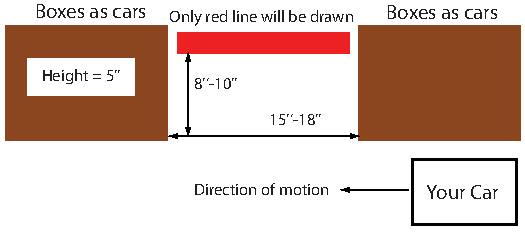
\includegraphics[angle=0, height=1.75in]{figures/lab4_parallel_park2.pdf}
%  \includegraphics[angle=0, height=2.0in]{figures/lab4_parallel_park.pdf}
\end{center}
 \caption{Course with dimensions. The actual distance, breadth and width, between parked cars will be decided on grading day. But it will be within the dimension range specified above.}
   \label{fig:lab4-course}
\end{figure}

\paragraph{Scoring} 
%The grading will take place in the classroom. Please arrive by 1:15 PM and be ready to demonstrate your robot. Ensure that the batteries are charged. 
%\subsection{Before you show up at the BSE atrium}
%\begin{enumerate}
%\item On grading day, the TA/instructor will have a different course with similar level of difficulty.
%\item 
One person from each team will place the robot at the start line as shown in the figure~\ref{fig:lab4-grading}. When the TA/instructor says, `Ready-Set-Go', the team member will press a button on the brick to get the robot moving. Your time will start when the TA/instructor says `Go'. {\bf Your robot should come to a complete stop when it thinks it has parallel parked itself. The robot  should also blink the red led on the programmable brick. We will stop the time once we see red light.}
%By default we will award 80 points to you and cancel points based on missed targets Points are deducted based on missed targets. 
The grading rubric is as follows:
\begin{enumerate}
\item If you do not follow the parallel parking convention (see notes above) then your score will be zero for that particular attempt. 
%\item{20 points:} As long as you drive and pull yourself parallel to the car near the intermediate point and then reverse to start the parking maneuver. If you do not do this maneuver then you will get zero points for the rest of the lab. 
\item {$T_1$ = 20 x 3 = 60 points:} For: (1) not hitting the front car; (2) not hitting the rear car; (3) not crossing the horizontal red line.
\item {$T_2$ = 20 points:} In the final stopping position, {\bf at least one tire is on the red line}. It is fine to be partially on the line. 
\item {$T_3$ = 20 points:} In the final stopping position, {\bf the orientation of the midline of the car is parallel to the horizontal red line}. To check alignment on a four wheeled car, we will check to see if the front/back tires on one side of the car are on the red line. If you use a single castor wheel then we will check to see if the orientation of the midline is within $\pm$ $5$ degrees of the red line (this is left to the discretion of the teaching assistant)
\item Final score = $T_1+T_2+T_3$ - Total time taken (in seconds).
%\item{10 points:} For parallel parking in under 30 seconds.
\item You will have three attempts to improve your scores. 
%\item The TA will record your score and the time taken. In order to be declared a winner, the team that scores 100 points and takes least amount of time is the winner. 
%\item Only 1 team from the entire classroom will be eligible to win the grand prize. 
\end{enumerate}
NOTE: The TA/instructors decision is final when making a judgement on the interpretation of any of these rules. 
%Here is a parking red line for testing (print on letter size paper): \\ \bluehref{http://aux.coe.utsa.edu/~pab/info/lego/lego\_park\_line.pdf}{http://aux.coe.utsa.edu/~pab/info/lego/lego\_park\_line.pdf}.
\begin{figure}[t]
\begin{center}
 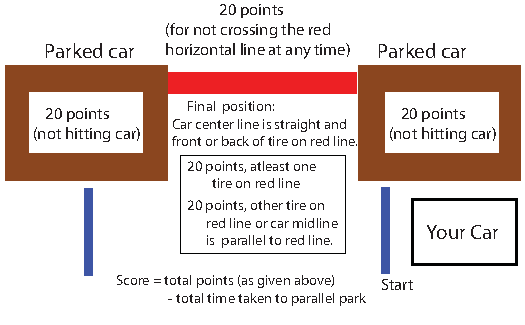
\includegraphics[angle=0, height=2.0in]{figures/lab4_parallel_park4.pdf}
\end{center}
 \caption{Explanation of grading for the lab.}
   \label{fig:lab4-grading}
\end{figure}
%Points will be awarded for reaching each of the check points in that order. If the robot skips a checkpoint but return to the line afterwards, you will not be awarded points from there on. TA/instructor decisions are final.
%The total score for this part is 80 points. You have to complete the entire course in 20 seconds. If your robot takes more than 20 seconds, then there is a 20 points penalty. {\bf (80 points)}.
%\item {\bf [20 points]}  Lab report (per group) is due by the end of the day the lab is graded.  Suggested report size is 2 pages, but a maximum of 5 pages is allowed. Please include a concise description of the problem and your solution, including lessons learnt (you will be able to do this after the lab is graded). {\bf Also we will give major emphasis on these two things so please ensure you have them in the write up: (1) make a table with two columns, one column should list the sensors while the second should list the purpose, and (2) draw flowchart depicting the logic used in your program.} Please do not copy-paste your code in the report. If you want, you can include small snippets of your code in the report but keep please keep it to a minimal. Photos, picture, drawings (sketches), link to explain your solution are highly encouraged. Email the file to pranav.bhounsule@utsa.edu. %NOTE: Please look at some example lab reports posted on blackboard. Please go through them and my comments for the report. Please use them as a template to help you write the report for this lab. %Grading will be stricter this time.
%%{\bf (20 points)}.
%\end{enumerate}

\section*{Packing up}
Please dis-assemble the robot and put contents in the correct location in the box. Please ensure that parts, sensors, motors, brick, {\bf cables}, {\bf usb cables} are returned to the box. The complete list is in the handout for yesterday which can be found here: \bluehref{http://tiny.cc/ieee\_day1}{http://tiny.cc/ieee\_day1}. Please hand over the box to the teaching assistant.

\end{document}